\documentclass[letterpaper,12pt]{article}
\usepackage{tabularx} % extra features for tabular environment
\usepackage{amsmath}  % improve math presentation
\usepackage{amsfonts}
\usepackage{verbatim}
\usepackage{graphicx} % takes care of graphic including machinery
\usepackage[margin=1in,letterpaper]{geometry} % decreases margins
\usepackage{cite} % takes care of citations
\usepackage[final]{hyperref} % adds hyper links inside the generated pdf file
\hypersetup{
	colorlinks=true,       % false: boxed links; true: colored links
	linkcolor=blue,        % color of internal links
	citecolor=blue,        % color of links to bibliography
	filecolor=magenta,     % color of file links
	urlcolor=blue         
}
\usepackage{blindtext}

\usepackage{units}
\usepackage{lineno}
%++++++++++++++++++++++++++++++++++++++++


\begin{document}
\linenumbers
\title{Uncertain Effects of DFT Functionals on Time-of-flight Calculations of Organic semiconductor }
\author{authors}
\date{\today}
\maketitle

\begin{abstract}
In this paper, the time-of-flight (ToF) is used to quantify the charge mobility in OSC. 
Using ToF as the quantity of interest, the uncertainty effect of the DFT functionals on the ToF in a BCP device is studied. 
Using a total of 10 different DFT functionals, we find that the electronic structure properties have similar distributions as indicated by Wasserstein distance, while the ToF can have a relatively large deviation.
Further investigation reveals that ToF can be sensitive to the energy of a single molecule, leading to the ToF being sensitive to DFT functionals.

Further investigation reveals that the BHANDHLYP functional leads to a trap site, and the charge mobility is very sensitive to the trap sites' energy, so a small change in the site's energy results in a large deviation of ToF.  
We further estimate the charge mobility distribution due to the uncertainty in electronic structure properties, and those properties' uncertainty is obtained from the maximum likelihood estimation of the 10 data points calculated using the 10 DFT functionals.
Ultimately, a confidence level of charge mobility is obtained, and it is found that the uncertainty in site energy has the most significant effect on the ToF. 
\end{abstract}

\section{Introduction}
Random walk in random environments is often used to model physical processes taking into account the varying disorder levels and environmental factors that influence the walker's movement. 
These disorders and environmental factors can introduce a level of uncertainty that significantly impacts the overall rates of the random walk, ultimately affecting the quantities of interest one aims to obtain.

A specific type of random walk in random environments is the charge transport in organic semiconductors (OSC), which consists of the amorphous mesoscopic structure due to spatially disordered molecular arrangement. 
Such structural disorder translates into electronic structure disorder, including energy disorder and coupling element disorder, which eventually leads the charge transport processes to be modeled as continuous time random walks (CTRWs). By representing the molecule as vertexes, the edge weights are assigned as the transition rates between the corresponding molecules, and the charge carriers are random walkers. 
The uncertainty brought by electronic structure disorder and environmental factors is reflected in the transition rates, that is the edge weights of the CTRWs. 

While the transition rates in those CTRWs can be calculated in a first-principle multiscale approach, this method involves some level of approximations. 
Since the charge transport in OSC involves electrons, quantum mechanics and Schr\"odinger equation are essential in providing a time-series behavior of the charge dynamics. 
But due to the complexity of Schr\"odinger Equation, one alternative theory is the density functional theory (DFT). DFT has two challenges. Firstly, it is computationally impossible to perform electronic structure calculations for the whole OSC device. And secondly, the exchange-correlation potential in DFT has an unknown formula.

The first challenge is overcome by approximating the electron dynamics as transition processes between the localized states, with the transition rates calculated as the temperature-activated bi-molecule transition rates, known as the Marcus rate. 
The second challenge is addressed by utilizing DFT functionals to represent the exchange-correlation potential. 
While there are benchmark results concerning the molecular energy calculation using different DFT functionals as well as rich literature on charge transport in the multiscale model OSC, a quantitative study of DFT functionals' effect on the charge transport processes is missing. 
Also missing is the influence of the uncertainty in the electronic structure properties on the quantity of interest. 

There are many challenges for this investigation. Firstly, due to the number of molecules ($\sim 1000$), since the CTRWs are usually of high dimensions, quantifying uncertainty in such high dimensions is numerically challenging. Secondly, simulating the CTRWs process itself can be a computationally challenging task due to some convergence issues.
Last but not least, the exact DFT functionals are not known so as the distribution of the transition rates for any two specific molecules. 

One of the main quantities of interest to characterize the charge transport in OSC is charge mobility. Using this as the quantity of interest,
the goal of this work is to investigate how the DFT functionals affect the electronic structures and charge mobility. The uncertainty due to the environmental factors that cause a change in the molecules' position is not considered in this work, although this topic itself is very important.
We want to answer the following questions: 
\begin{itemize}
    \item How do DFT functionals change the reorganization energy, distribution of molecule energies and coupling elements? 
    \item How do DFT functionals change the charge mobility?
    \item Which electronic structure (among energy, coupling element and reorganization energy) has the most impact on the uncertainty of charge mobility?
    \item Can we estimate the range of the quantity of interest, given a confidence level?
\end{itemize}

With an external electric field, the charge mobility can be calculated as $\mu = \frac{\vec{v} \vec{F}}{|\vec{F}|^2}$ where $\vec{v}$ is the average drift-diffusive velocity of the charge carrier(s).
Without an electric field, $\vec{v}$ is the purely diffusive velocity. 
In electronic devices, the velocity is obtained from \textit{time-of-flight} (ToF) experiments, where charge carriers are injected into the cathode and collected at the anode. The ToF, denoted as $\tau$, is the period from injection to detection of at least one charge carrier. 
Then the velocity is simply $|\vec{v}| = \frac{L}{\tau}$, where $L$ is the length of the sample, which is usually chosen to be along the electric field direction if there is any. 

Analogously, the ToF calculation for multiscale modeled OSC sets up some molecules as \textit{Source} and some as \textit{Sink}. The key quantity for characterizing the charge transport, especially for uncertainty quantification, is the ToF, since the sample length $L$ is fixed and can be seen as a constant. 

In literature regarding multiscale modeled OSC, most works on charge transport reported steady-state charge mobility. This setting repeats the molecule graph infinitely in all three dimensions by periodic boundary conditions. Then, the CTRWs on the graph are simulated, usually by kinetic Monte Carlo numerically. However, this method suffers from challenges such as convergence issues. Namely, there is no guarantee that the number of Monte Carlo simulations will correctly present the charge carrier occupation in each molecule, and this becomes a problem if we want to calculate some quantities for a confidence level. 

Therefore, the charge mobility based on ToF is the focus to characterize charge transport.
Specifically, diffusive ToF with one charge carrier is used as the quantities of interest, and its calculation is based on the hitting time of a continuous time Markov chain. 
Diffusive ToF only considers electronic structures, without the influence of external electric fields, making clear the sensitivity effect path starting from DFT functional to electronic structures and eventually to ToF mobility. 
We only consider the CTRWs with one charge carrier, since multiple charge carriers will lead to a huge dimension, making the uncertainty quantification difficult to approach computationally, plus other issues. Also, since we only simulate a very limited-size system, using only one charge carrier is aligned with the low carrier density at the electric device level. 
Furthermore, multiple charge carriers will effectively disable some low-energy molecules which are important in uncertainty quantification. 

%%%%%%%%%%%%%%%%%%%%%%%%%%%%%%%%%%%%%%%%
\section{Multiscale Model}
\label{sec:MSM}
To perform multiscale modeling, the BCP (dimethyl-diphenyl-1,10-phenanthroline) device is used as the OSC in this work, since BCP has small conductivity and has been used as hole-trapping materials \cite{tsung_carrier_2008}.
A BCP device consisting of 1000 molecules is shown in Fig.\ref{fig:ToFFill}(b) with atomistic details.

%\begin{figure}
%    \centering
%    \includegraphics[width=0.4\textwidth]{figs/BCP_trap.png}
%   \caption{ BCP device simulated from MD. The Source and Sink molecules are highlighted by the blue color, and the molecule corresponding to node 66 is highlighted by the red color. The other BCP molecules are in grey. }
%   \label{fig:BCP}
%\end{figure}

The atomistic coordinates as well as the center-of-mass (COM) of each BCP molecule are generated from atomistic Molecular dynamics simulation, whose details are given in the Appendix.
For modeling purposes, this molecular system is modeled as a graph on which the random walk takes place. Each vertice represents a molecule, which also corresponds to a localized state mentioned in the introduction. 
Using a cutoff distance $r_\text{cutoff}$, any two molecules whose COM is within $r_\text{cutoff}=0.5$ [nm] are connected by directed edges with a weight $\omega_{i,j}$, and usually $\omega_{i,j} \neq \omega_{j,i}$.
The directed edge weights $\omega_{i,j}$ takes the electron transfer rate from localized state of molecule $i$ to that of molecule $j$, commonly expressed as Marcus rate:
%
\begin{equation}
    \omega_{ij} = \frac{2\pi}{\hbar} \frac{|J_{i,j}|^2}{\sqrt{4\pi \lambda_{i,j} k_\text{B}T}} \exp\left(-\frac{(\Delta E_{i,j} + q \cdot \vec{r}_{i,j} - \lambda_{i,j})^2}{4\lambda_{i,j} k_\text{B}T}\right) ,
    \label{equ:Marcus}
\end{equation}
%
where $\hbar$ is the reduced Planck constant, $k_\text{B}$ the Boltzmann constant. The temperature $T$ (in \unit[]{K}), and the charge of the carrier $q$ (in \unit[]{e}) can be considered as parameters of the simulation. The vector $\vec{r}_{i,j} = (r^x_{ij},r^y_{ij},r^z_{ij})^\text{T}$ connects the center-of-masses of molecules $i$ and $j$, which is calculated cyclic boundary conditions depending on the boundary condition.
The remaining quantities are calculated for each molecule using principles from quantum mechanics and classical mechanics: the reorganization energy $\lambda_{i,j}$, the electronic coupling $J_{ij}$, and the energy difference $\Delta E_{i,j} = E_i - E_j$ (all in \unit[]{eV}). 

In summary, the multiscale model for ToF calculation refers to the process: Firstly, classical Molecular Dynamics is used to generate the atomistic coordinates from which the vertex and edge sets are defined,
secondly, quantum electronic structure calculation is performed to obtain the parameter sets $\left\{\lambda_{i,j}\right\}$,  $\left\{J_{ij}\right\}$, and $\left\{\Delta E_{i,j}\right\}$ based on the atomistic details to define the edge weights. Finally from those parameters, ToF is evaluated.
In the remaining section, we will introduce the calculation details of $\left\{\lambda_{i,j}\right\}$,  $\left\{J_{ij}\right\}$, $\left\{\Delta E_{i,j}\right\}$ and ToF. 

\subsection{Electronic Structure Calculation} 
Each molecule is an $N_\text{el}$-electron system, and in quantum mechanics, the probability of finding electrons in space is described by the wavefunction.
The energy eigenvalue from the standard Kohn–Sham model \cite{kohn_self_1965} for a molecule (consisting of electrons and nuclei) reads:
\begin{equation}
    E_0 = \text{inf}\{ E^\text{KS}(\psi),\psi=(\phi_1,\cdots,\phi_{N_\text{el}}) \in (L_2(\mathbb{R}^3))^N, \int_{\mathbb{R}^3} \phi_i \phi_j =\delta_{ij} \} 
    \label{eq:KS_model}
\end{equation}
where the single-electron wavefunction $\phi_i$ satisfies $(-\frac{1}{2}\nabla^2_\mathbf{r} + \hat{V}_\text{ext} + \hat{V}_\text{H}[\rho] + \hat{V}_\text{XC}) \phi_i^\text{KS} =  E^\text{KS}_i[\rho] \phi^\text{KS}_i$ with electron density $\rho$. 
The kinetic energy operator is $-\frac{1}{2}\nabla^2_\mathbf{r}$, external potential energy operator $\hat{V}_\text{ext}$ includes all electrostatic background potentials such as the nuclear potential of all the atoms.
The Coulomb interaction operator is $\hat{V}_\text{H}[\rho] = \int_{\mathbb{R}^3} \frac{\rho(\vec{r}')}{ |\vec{r} - \vec{r}'| }$, and Kohn-Sham energy $E^\text{KS}_i$ of electron $i$. The molecule wavefunction $\psi$ lives in squared integrable Lebesgue space $L_2(\mathbb{R}^3)$. 

The exchange-correlation operator $\hat{V}_\text{XC}$ accounts for all the nonclassical terms, namely, the potential and kinetic energy associated with electron exchange and correlation. Knowledge of the exact $\hat{V}_\text{XC}$ makes obtaining the exact energy eigenvalue of many-body ground state possible. However, the exact $\hat{V}_\text{XC}$ is unknown and approximations, such as local density approximation (LDA), generalized gradient approximation (GGA) or a mixture of those two approximations with other models, are used in practice as the form of DFT functionals. 
The ten DFT functionals are shown in Table \ref{tab:para}.

The energy eigenvalue $E_0$ depends on the atomic coordinates of the molecule. The optimized geometry of a molecule refers to the atomic coordinates that minimize $E_0$.
The reorganization energy $\lambda_{i,j}$ from molecule $i$ to molecule $j$ is given as:
\begin{equation}
    \lambda_{ij} = E_i^\text{nC} - E_i^\text{nN} + E_j^\text{cN} - E_j^\text{cC}
\end{equation}
where $E_i^\text{nC}$ is the energy eigenvalue of the neutral molecule $i$ with the optimized geometry of charged molecule. When charge carriers are holes, a charged molecule has one electron less compared to a neutral molecule. Similarly, $E_j^\text{cN}$ is the energy eigenvalue of the charged molecule with the optimized geometry of the neutral molecule. For the BCP device, we obtain $\lambda_{ij}=0.50$ eV since this is only one type of molecule.

The site energy $E_i$ is calculated by:
\begin{equation}
    E_i = (E_i^\text{cC} - E_i^\text{nN}) + E_i^\text{el}
    \label{eq:siteE}
\end{equation}
where $E_i^\text{nN}$ is single-point energy of the neutral molecule $i$ with the optimized geometry of neutral molecule. Similarly, $E_i^\text{cC}$ is the single-point energy of the charged molecule $i$ with the optimized geometry of the charged molecule. In physical interpretation, $E_i^\text{cC} - E_i^\text{nN}$ is the adiabatic ionization potential of molecule $i$.
And $E_i^\text{el}$ is the electrostatic interactions given by:
%
\begin{equation}
    E_i^\text{el} = \frac{1}{4 \pi \epsilon_0} \sum\limits_{a_i} \sum\limits_{b_k,k\neq i} 
    \frac{(q_{a_i}^\text{c} - q_{a_i}^\text{n}) q_{b_k}^\text{n}}{\epsilon_s r_{a_i,b_k}}
    \label{equ:Eel}
\end{equation}
%
where $i,k$ index molecules, $a_i$ and $b_k$ refer to atoms belonging to molecule $i,k$, $r_{a_i,b_k} = || \vec{r}_{a_i} - \vec{r}_{b_k} ||_2$ is the distance between atoms $a_i$ and $b_k$, and $\epsilon_s$ represents the static relative dielectric constant and is a function of the dipole moment of the molecule. From the atomic charges, the dipole moment is calculated via $\mu_i = \sum\limits_{a_i} q_{a_i} \cdot \vec{r}_{a_i}$. The molecule energies and their distribution are shown in the appendix.

%%%%%%%
The coupling element $J_{i,j}$ between molecule $i$ and $j$ is calculated \cite{baumeier_density_2010} using the electron wave function of the molecules obtained from the Kohn-Sham equation: 
\begin{equation}
    J_{i,j} = \frac{ J^0_{i,j}- \frac{1}{2}(e_i+e_j)\mathbf{S}_{i,j} }{ 1- \mathbf{S}_{i,j}^2 }
    \label{equ:JAB}
\end{equation}
where $J^0_{i,j} = \langle \psi^i | \hat{H} | \psi^j \rangle $, $e_i = \langle \psi^i | \hat{H} | \psi^i \rangle $, $e_j = \langle \psi^j | \hat{H} | \psi^j \rangle $, and $\mathbf{S}_{i,j}=\langle \psi^i | \psi^j \rangle $ with bra-ket notation, $\hat{H}$ is the Hamiltonian of the electron wave function, and $\psi^{i,(j)}$ is the electron wave function of molecule $i(j)$. A single molecule is called a monomer, and a pair of two molecules is called a dimer.

Denote $\psi^\text{D}$ as the electron wave function of the two molecules,  $J^0_{i,j}$ can be calculated via:
$
    J^0_{i,j} = \mathbf{\gamma}^i \text{diag}(\mathcal{E}) \mathbf{\gamma}^j
$, 
where $\mathbf{\gamma}^i = \langle \psi^i | \psi^\text{D} \rangle$ and $\mathbf{\gamma}^j = \langle \psi^j | \psi^\text{D} \rangle$ are called the projections of the monomer orbitals $\psi^i, \psi^j$ on the dimer orbitals $\psi^\text{D}$. And $\text{diag}(\mathcal{E})$ is the diagonal matrix consisting of energy eigenvalues of the one-particle wave function of the dimer. The molecular coupling element distribution is shown in the appendix.


\section{Time-of-flight Calculation}
After defining the graph $\mathbf{G}=(\mathbf{W},\mathbf{E})$ and calculating the edge weights from the multiscale model, the charge dynamics can be modeled as a continuous-time random walk process on the graph. 
To model the Source-Sink conditions in many devices such as the neuromorphic devices mentioned in the introduction, some vertices are used as \textbf{Source} to represent the electrode where charge carriers are injected, and some vertices as \textbf{Sink} where charge carriers are detected and ToF recorded.
Due to Coulomb repulsion, each node can be occupied by one charge carrier at most, so a system with $N$ molecules and $N_c$ charge carriers has a total of $C^N_{N_C}$ occupation situations. Each of these occupation situations is considered as a state $\mathbf{s}$. 
If all the carriers' occupations are in the Source node, the state is called the Source state, and if at least one of the Sink nodes is occupied, the state is called the Sink state. 
The transition rates between the states can be obtained from the adjacency matrix $\mathbf{W}:\omega_{i,j}$, since the connectivity of states is encoded in the connectivity of the nodes, as detailed in ~\cite{chen_graph_2024}. 
According to such connectivity, 
the transition rates $\Omega_{\mathbf{s} \mathbf{s}' }$ from state $\mathbf{s}$ to $\mathbf{s}'$ is:
\begin{equation}\label{eq:transition_rates}
	\Omega_{\mathbf{s} \mathbf{s}^\prime} =
	\begin{cases}
	     0			&  \mathbf{s} \text{ is not connected to } \mathbf{s}^\prime,\\
	    \omega_{ij}	&  \mathbf{s} \text{ is connected to } \mathbf{s}^\prime \text{ due to } (i,j)
	\end{cases}
\end{equation}

Then the transition probability from state $\mathbf{s}$ to $\mathbf{s}'$ is $p_{\mathbf{s} \mathbf{s}^\prime} = \Omega_{\mathbf{s} \mathbf{s}^\prime}/D_\mathbf{s}$ where $D_\mathbf{s} := \sum_{\mathbf{s}^\prime \ne \mathbf{s}} \Omega_{\mathbf{s} \mathbf{s}^\prime}$.
And the expected time from state $\mathbf{s}$ to reach the Sink state $\tau_\mathbf{s}$ is calculated 
~\cite{chen_graph_2024} via: 
\begin{equation}\label{eq:hitting_time}
	\tau_\mathbf{s} = \begin{cases}
		\frac{1}{D_\mathbf{s}} + \sum_{\mathbf{s}^\prime \ne \mathbf{s}} p_{\mathbf{s} \mathbf{s}^\prime} \tau_{\mathbf{s}^\prime} &\text{if $\mathbf{s}$ is not a sink state},\\
		0 &\text{else.} 
	\end{cases}
\end{equation} 

Since we need to consider all possible starting nodes of the carriers, all the Source states need to be considered. 
The random walk process has been modeled as a parallel electric network of capacitors~\cite{doyle_random_2000}, and accordingly, we evaluate the ToF to be the harmonic mean:
%
\begin{equation}
\tau = N_\text{source} \left[\sum_{\mathbf{s}\in \text{source}} (\tau_\mathbf{s}^\ast)^{-1}\right]^{-1},
\end{equation}
with $N_\text{source}$ the number of source states.

%%%%%%%%%%%%%%%%%%%%%%%%%%%%%%%%%%%%%%%
\section{Results}
\label{sec:result}

\subsection{Distribution Distance and ToF Differences}
A summary of the Time-of-Flight (ToF) and molecular energies using different functionals is provided in Table \ref{tab:para}, with the drift ToF detailed in Table \ref{tab:para2}. The tables indicate that while the energy standard deviations $\sigma(E)$ are similar across different functionals, the ToF values vary significantly, notably for functionals like BHANDHLYP, M06L, and BHLYP.

\begin{table}[h]
    \centering
    \begin{tabular}{c c c c c }
    \hline
        Functional & ScaleHFX & $\lambda_h$ [eV] & ToF [s] & $\sigma(E)$ \\ 
        \hline
        PBE0 & 0.25 & 0.388 & 1.23e-3 & 0.175 \\
        PBE & 0 & 0.303 & 1.04e-3 & 0.172 \\ 
        B3LYP & 0.20 & 0.375 & 4.28e-3 & 0.175 \\
        BHANDHLYP & 0.5 & 0.494 & \textbf{737.94} & 0.192 \\
        TPSS & 0 & 0.310 & 1.37e-2 & 0.168 \\
        BP86 & 0 & 0.304 & 7.46e-3 & 0.175 \\
        wB97X & 0.157 & 0.505 & 2.92e-2 & 0.191 \\
        wB97X-D3 & 0.195 & 0.496 & 4.89e-2 & 0.180 \\
        M06L & 0 & 0.312 & 3.19e-1 & 0.165 \\
        BHLYP & 0.5 & 0.493 & 2.47 & 0.192 \\
    \hline
    \end{tabular}
    \caption{Values of $\lambda_h$, ToF, stationary state velocity, and energy standard deviation of BCP molecules calculated from different functionals.}
    \label{tab:para}
\end{table}

\begin{table}[h]
    \centering
    \begin{tabular}{c c c}
    \hline
        Functional & ToF [s] & $\mu$ [m/s] \\ 
        \hline
        PBE0 & 2.39e-8 & 5.68e-5 \\
        PBE & 6.03e-9 & 2.25e-4 \\ 
        B3LYP & 1.67e-8 & 8.13e-5 \\
        BHANDHLYP & 3.36e-4 & 4.04e-9 \\
        TPSS & 1.23e-8 & 1.10e-4 \\
        BP86 & 3.77e-7 & 3.59e-6 \\
        wB97X & 1.68e-6 & 8.08e-7 \\
        wB97X-D3 & 6.92e-7 & 1.96e-6 \\
        M06L & 3.90e-3 & 3.47e-10 \\
    \hline
    \end{tabular}
    \caption{Mobility and ToF with drift electric field $6 \times 10^7$ V/m.}
    \label{tab:para2}
\end{table}

\textbf{Point 1:} To investigate the effect of different functionals $f^\text{DFT}$ on electronic structures, we compare the energies $E_i$ and couplings $J_{i,j}$ for all molecule indices $i,j$. Scatter plots in Figures \ref{fig:scatterE} and \ref{fig:scatterJ} illustrate these comparisons.

\begin{figure}[h]
    \centering
    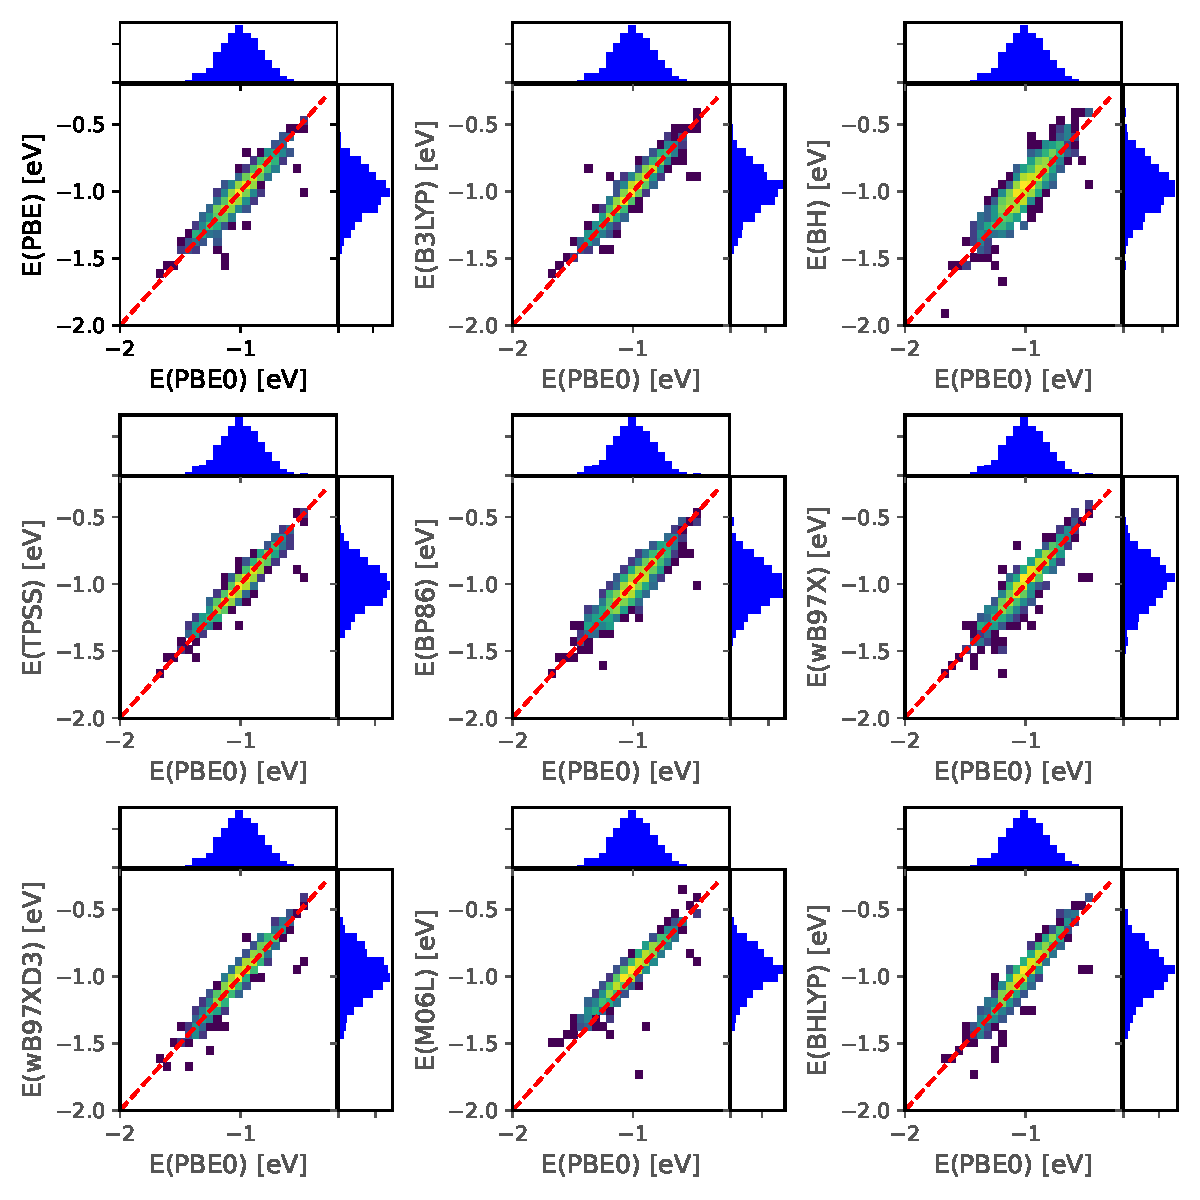
\includegraphics[width=0.95\textwidth]{figs/scatterE_all.pdf}
    \caption{Energy heat maps: $X$-axis shows energies of BCP molecules obtained using PBE0, while the $Y$-axis shows energies from a different functional $f'$.}
    \label{fig:scatterE}
\end{figure}

\begin{figure}[h]
    \centering
    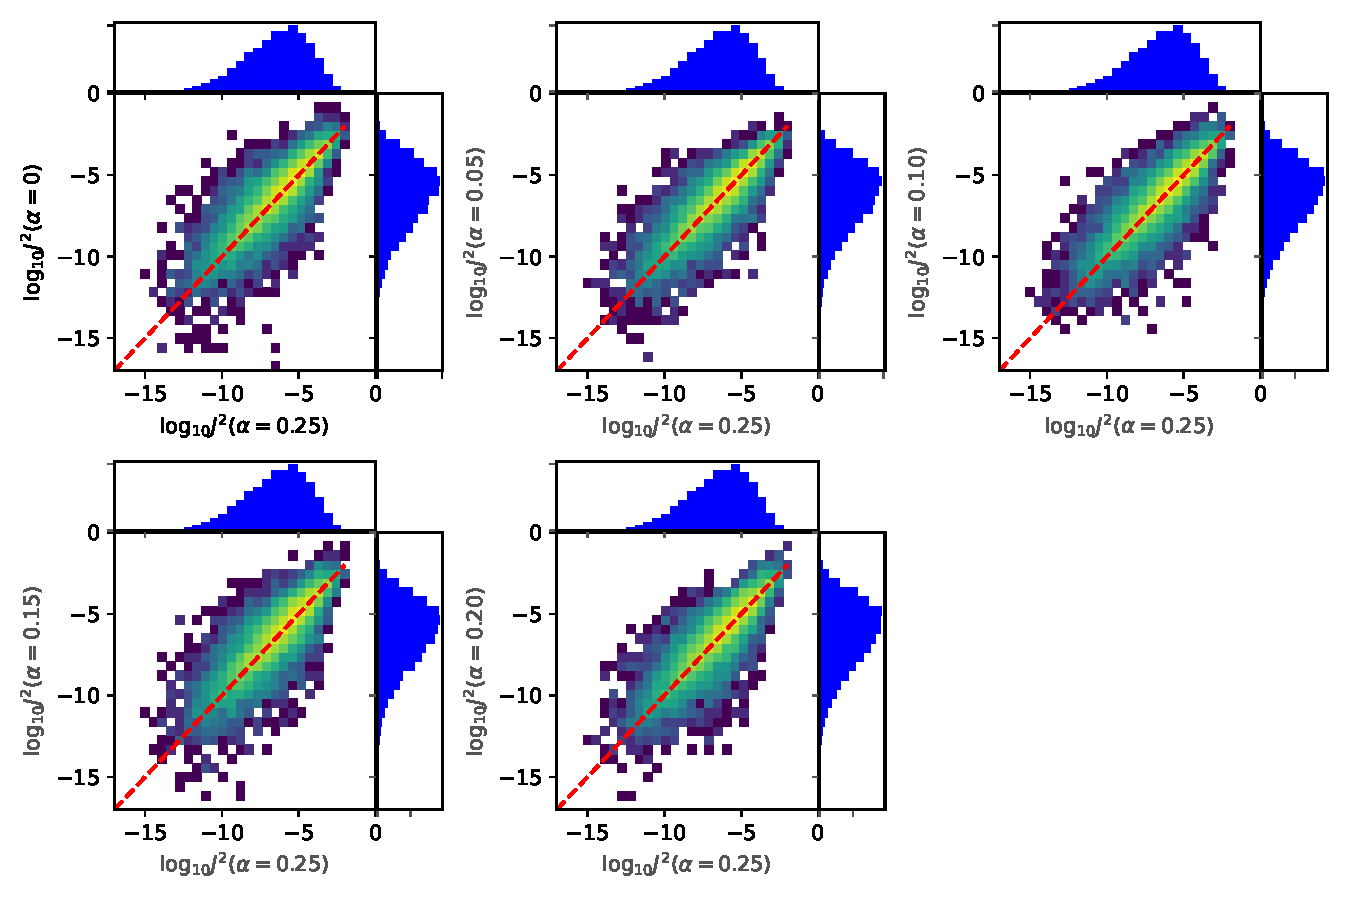
\includegraphics[width=0.95\textwidth]{figs/scatterJ_all.pdf}
    \caption{Scatter heat maps of $\log_{10}(J^2)$: $X$-axis shows $\log_{10}(J^2)$ of BCP molecules obtained using PBE0, while the $Y$-axis shows $\log_{10}(J^2)$ from a different functional $f'$.}
    \label{fig:scatterJ}
\end{figure}

\textbf{Point 2:} Both $E_i$ and $J_{i,j}$ are distributions. To quantify the impact of these distributions on $\Delta$ToF, we plot the Wasserstein distance versus $\Delta$ToF. Figure \ref{fig:distance_ToF} shows that different functionals generate similar energy sets, but $\Delta$ToF is not correlated with energy distribution distance.

\begin{figure}[h]
    \centering
    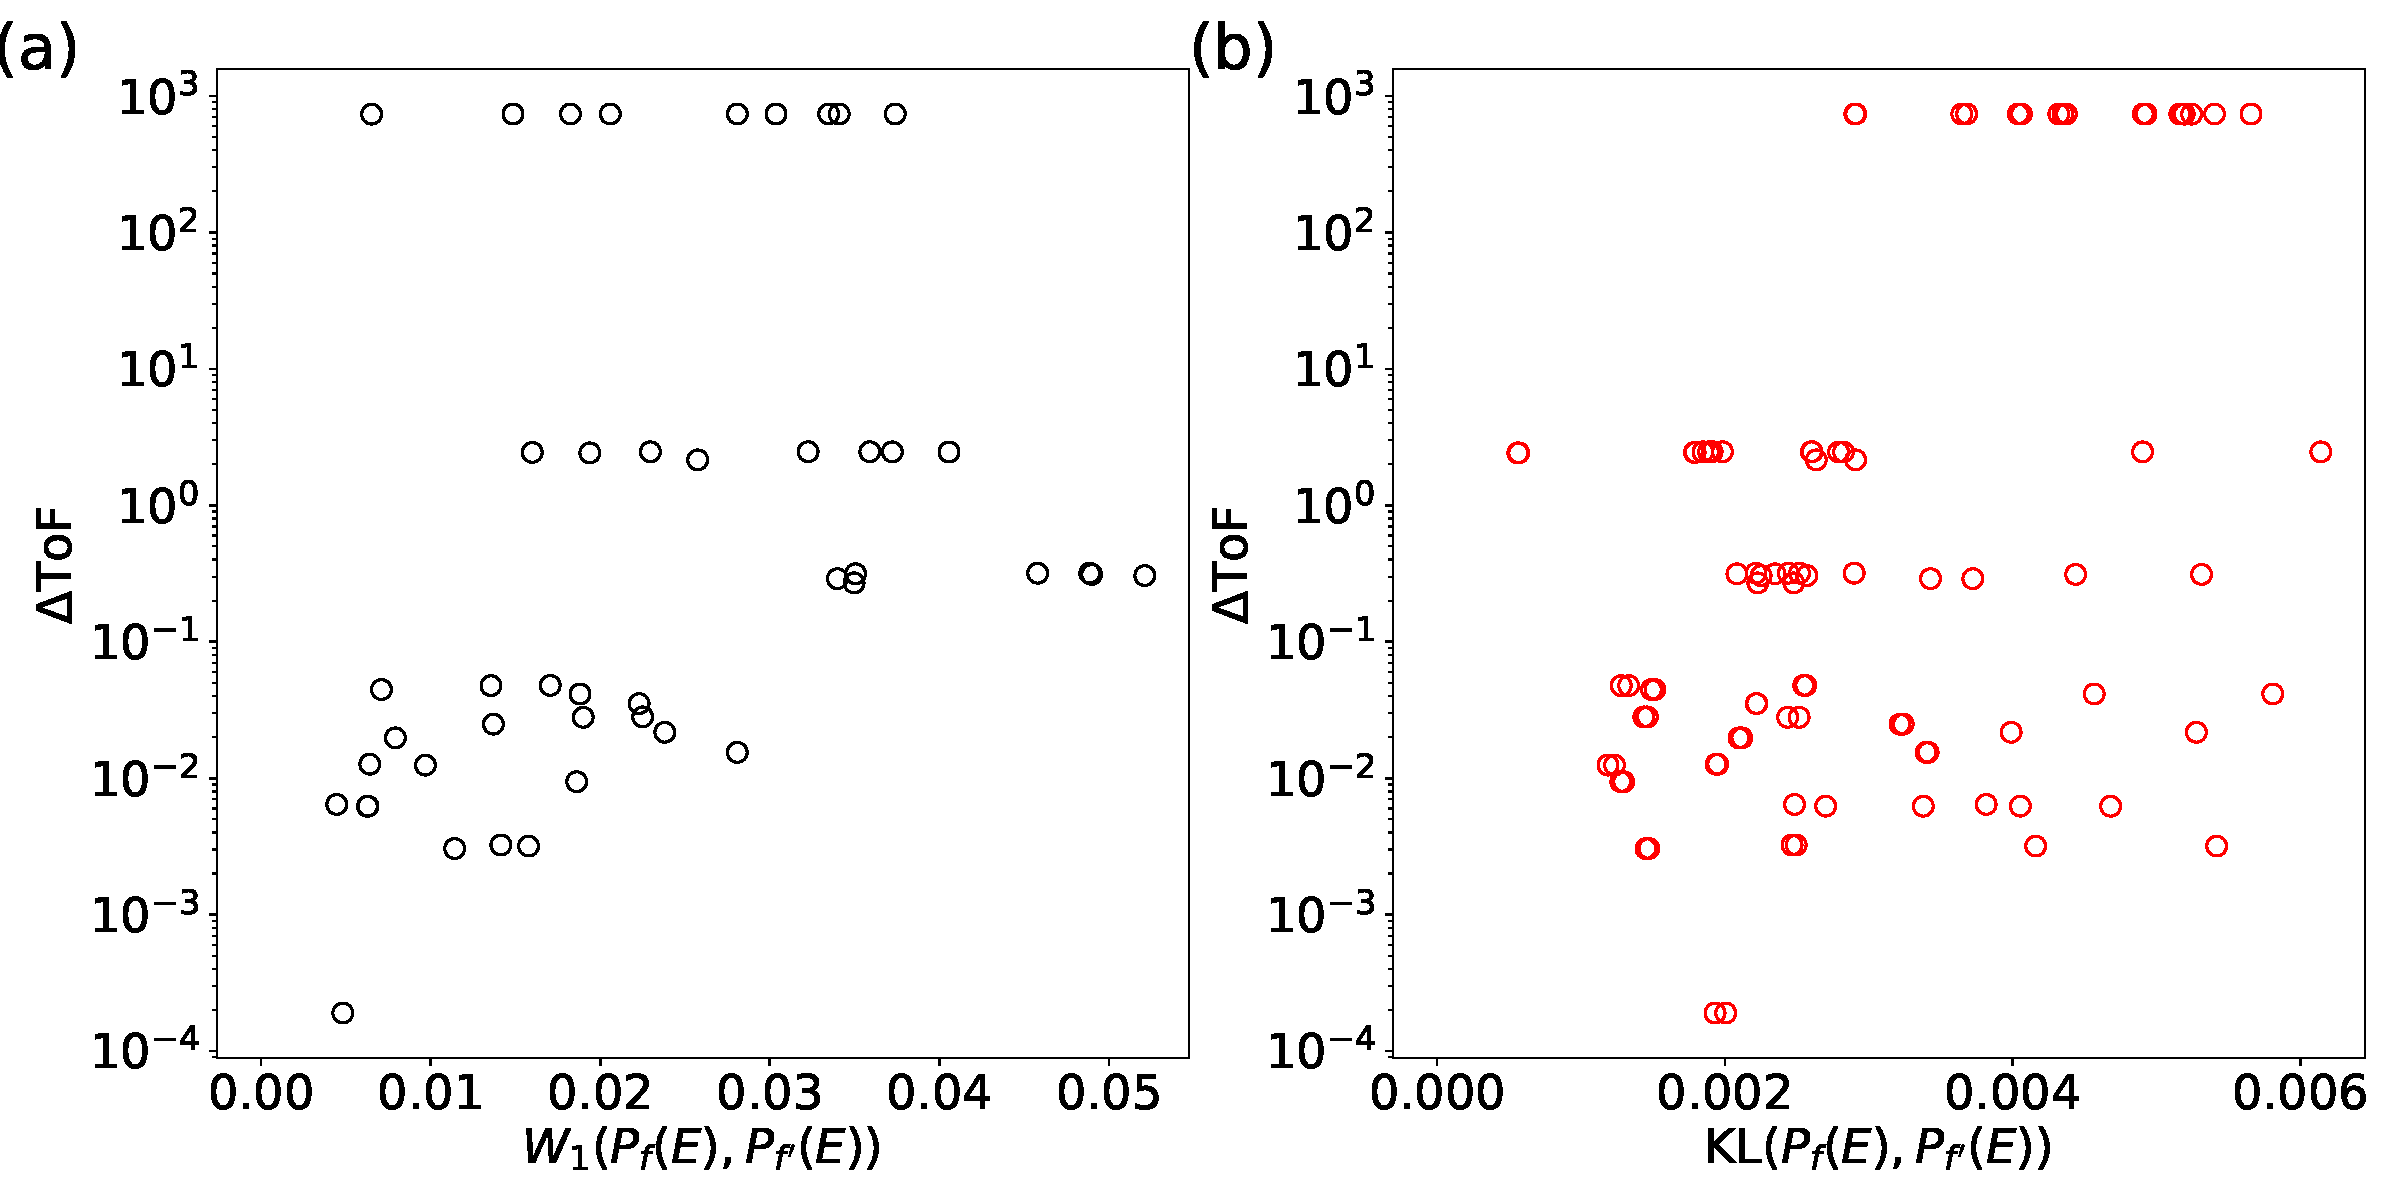
\includegraphics[width=0.9\textwidth]{figs/DeltaToF_W_KL_E.pdf}
    \caption{Left: scatter plot of $W_1(P_f,P_{f'})$ vs. $\Delta$ToF. Right: scatter plot of $KL(P_f(E),P_{f'}(E))$ vs. $\Delta$ToF.}
    \label{fig:distance_ToF}
\end{figure}

\textbf{Point 3:} We then examine other rate-related parameter distributions, calculating the Wasserstein distance and plotting against $\Delta$ToF. Figure \ref{fig:d_WD_tof} reveals that only the rate $P_f(\omega)$ has a large Wasserstein distance when varying $f^\text{DFT}$; other parameters show similar distributions.

\begin{figure}[h]
    \centering
    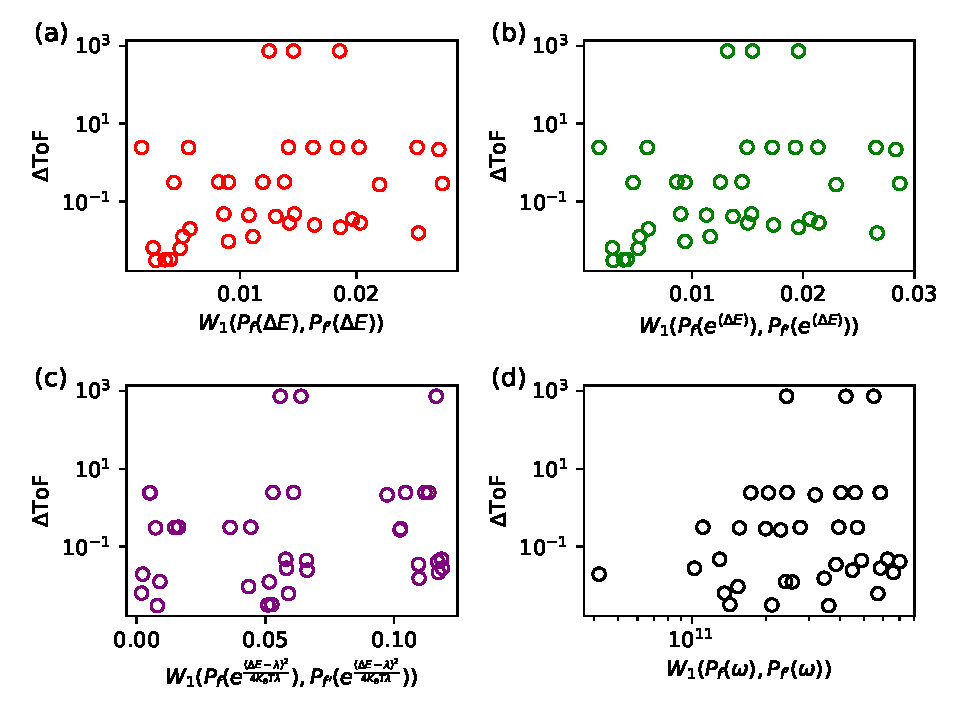
\includegraphics[width=0.7\textwidth]{figs/DeltaToF_W_all.pdf}
    \caption{Scatter plots of (a): $W_1(P_f(\Delta E),P_{f'}(\Delta E))$, (b): $W_1(P_f(\exp(\Delta E)),P_{f'}(\exp(\Delta E)))$, (c): $W_1(P_f(\exp \frac{-(\Delta E - \lambda)^2}{4 k_B T \lambda}),P_{f'}(\exp \frac{-(\Delta E - \lambda)^2}{4 k_B T \lambda}))$, and (d): $W_1 (P_f(\omega), P_{f'}(\omega) )$ vs. $\Delta$ToF.}
    \label{fig:d_WD_tof}
\end{figure}


\textbf{Point4:} Although $f^\text{DFT}$ affects $P_f(\omega)$, but we further notice that $\Delta$ToF is not correlated to its Wasserstein distance. 
So we hypothesize that the connectivity of the graph changed due to different $f^\text{DFT}$. The connectivity of the graph is quantified by the second eigenvector of the graph Laplacian, so we make the figure to investigate the correlation between the $\Delta$ToF and the graph connectivity. 
Figure .\ref{fig:d_eig_tof} shows the ratio of $f^\text{DFT}$ and the second eigenvalue ratio between the graph Laplacian. These two quantities look correlated, and we calculate the Spearman rank coefficient, which is shown in Table.\ref{tab:spearman}.

\begin{table}[h]
    \centering
    \begin{tabular}{c c c}
    \hline
        Data Set & Spearman Rank Coefficient & $p$-value \\ 
        \hline
        $\frac{\lambda_{2,L_W}(f)}{\lambda_{2,L_W}(f')}$ vs $\frac{\text{ToF}(f)}{\text{ToF}(f')}$ & -0.57 & 4.6e-5 \\
        $\frac{\lambda_{2,L_\text{rw}}(f)}{\lambda_{2,L_\text{rw}}(f')}$ vs $\frac{\text{ToF}(f)}{\text{ToF}(f')}$ & -0.38 & 9.4e-3 \\ 
    \hline
    \end{tabular}
    \caption{Spearman rank coefficients for the relationship between $\frac{\lambda_2(f)}{\lambda_2(f')}$ and $\frac{\text{ToF}(f)}{\text{ToF}(f')}$}
    \label{tab:spearman}
\end{table}

\begin{figure}[h]
    \centering
    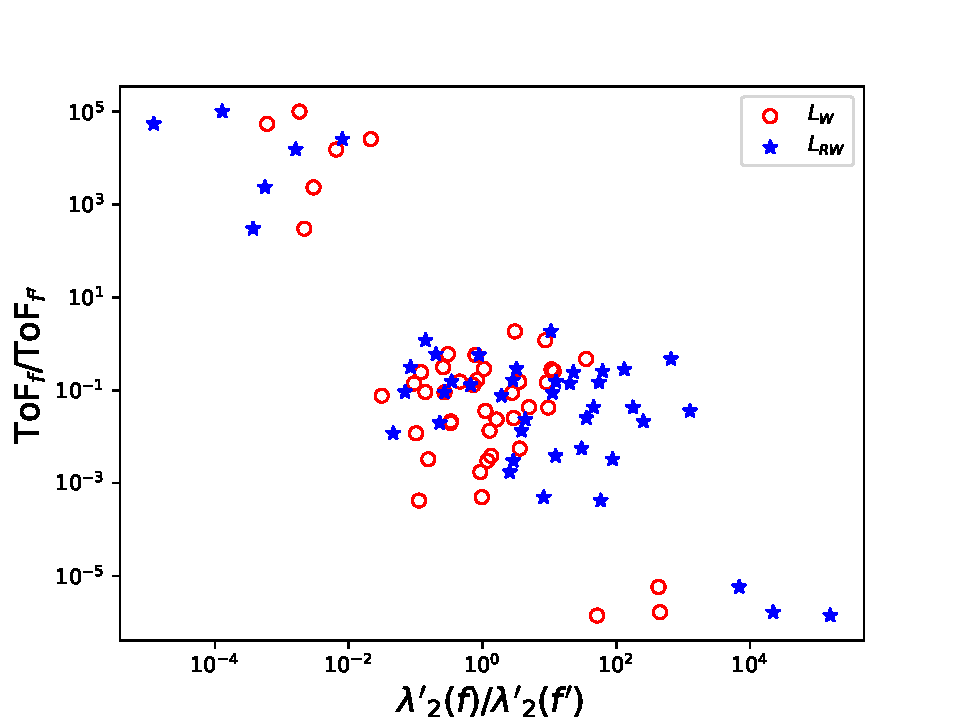
\includegraphics[width=0.6\textwidth]{figs/ratio_tof_2ndEigval.pdf}
    \caption{Scatter plot of $\frac{\lambda_{2}(f)}{\lambda_{2}(f')}$ vs. $\frac{\text{ToF}(f)}{\text{ToF}(f')}$}
    \label{fig:d_eig_tof}
\end{figure}


\textbf{Point5:} The eigenvalue comes in pair with the eigenvector, so we further investigated the corresponding second eigenvector element distributions, as shown in Fig.\ref{fig:2ndVecLW}. 
To our surprise, node 66 has very different second eigenvector entries, so we performed K-means partitioning on those second eigenvector elements.

\textbf{Point6:} After partitioning, we notice that the partition cost function is correlated to $\Delta$ToF.
This correlation shows that the $\Delta$ToF correlated to the connectivity of the graph, althouth the electronic structures and rate-related parameters are similar. 

\begin{figure}
    \centering
    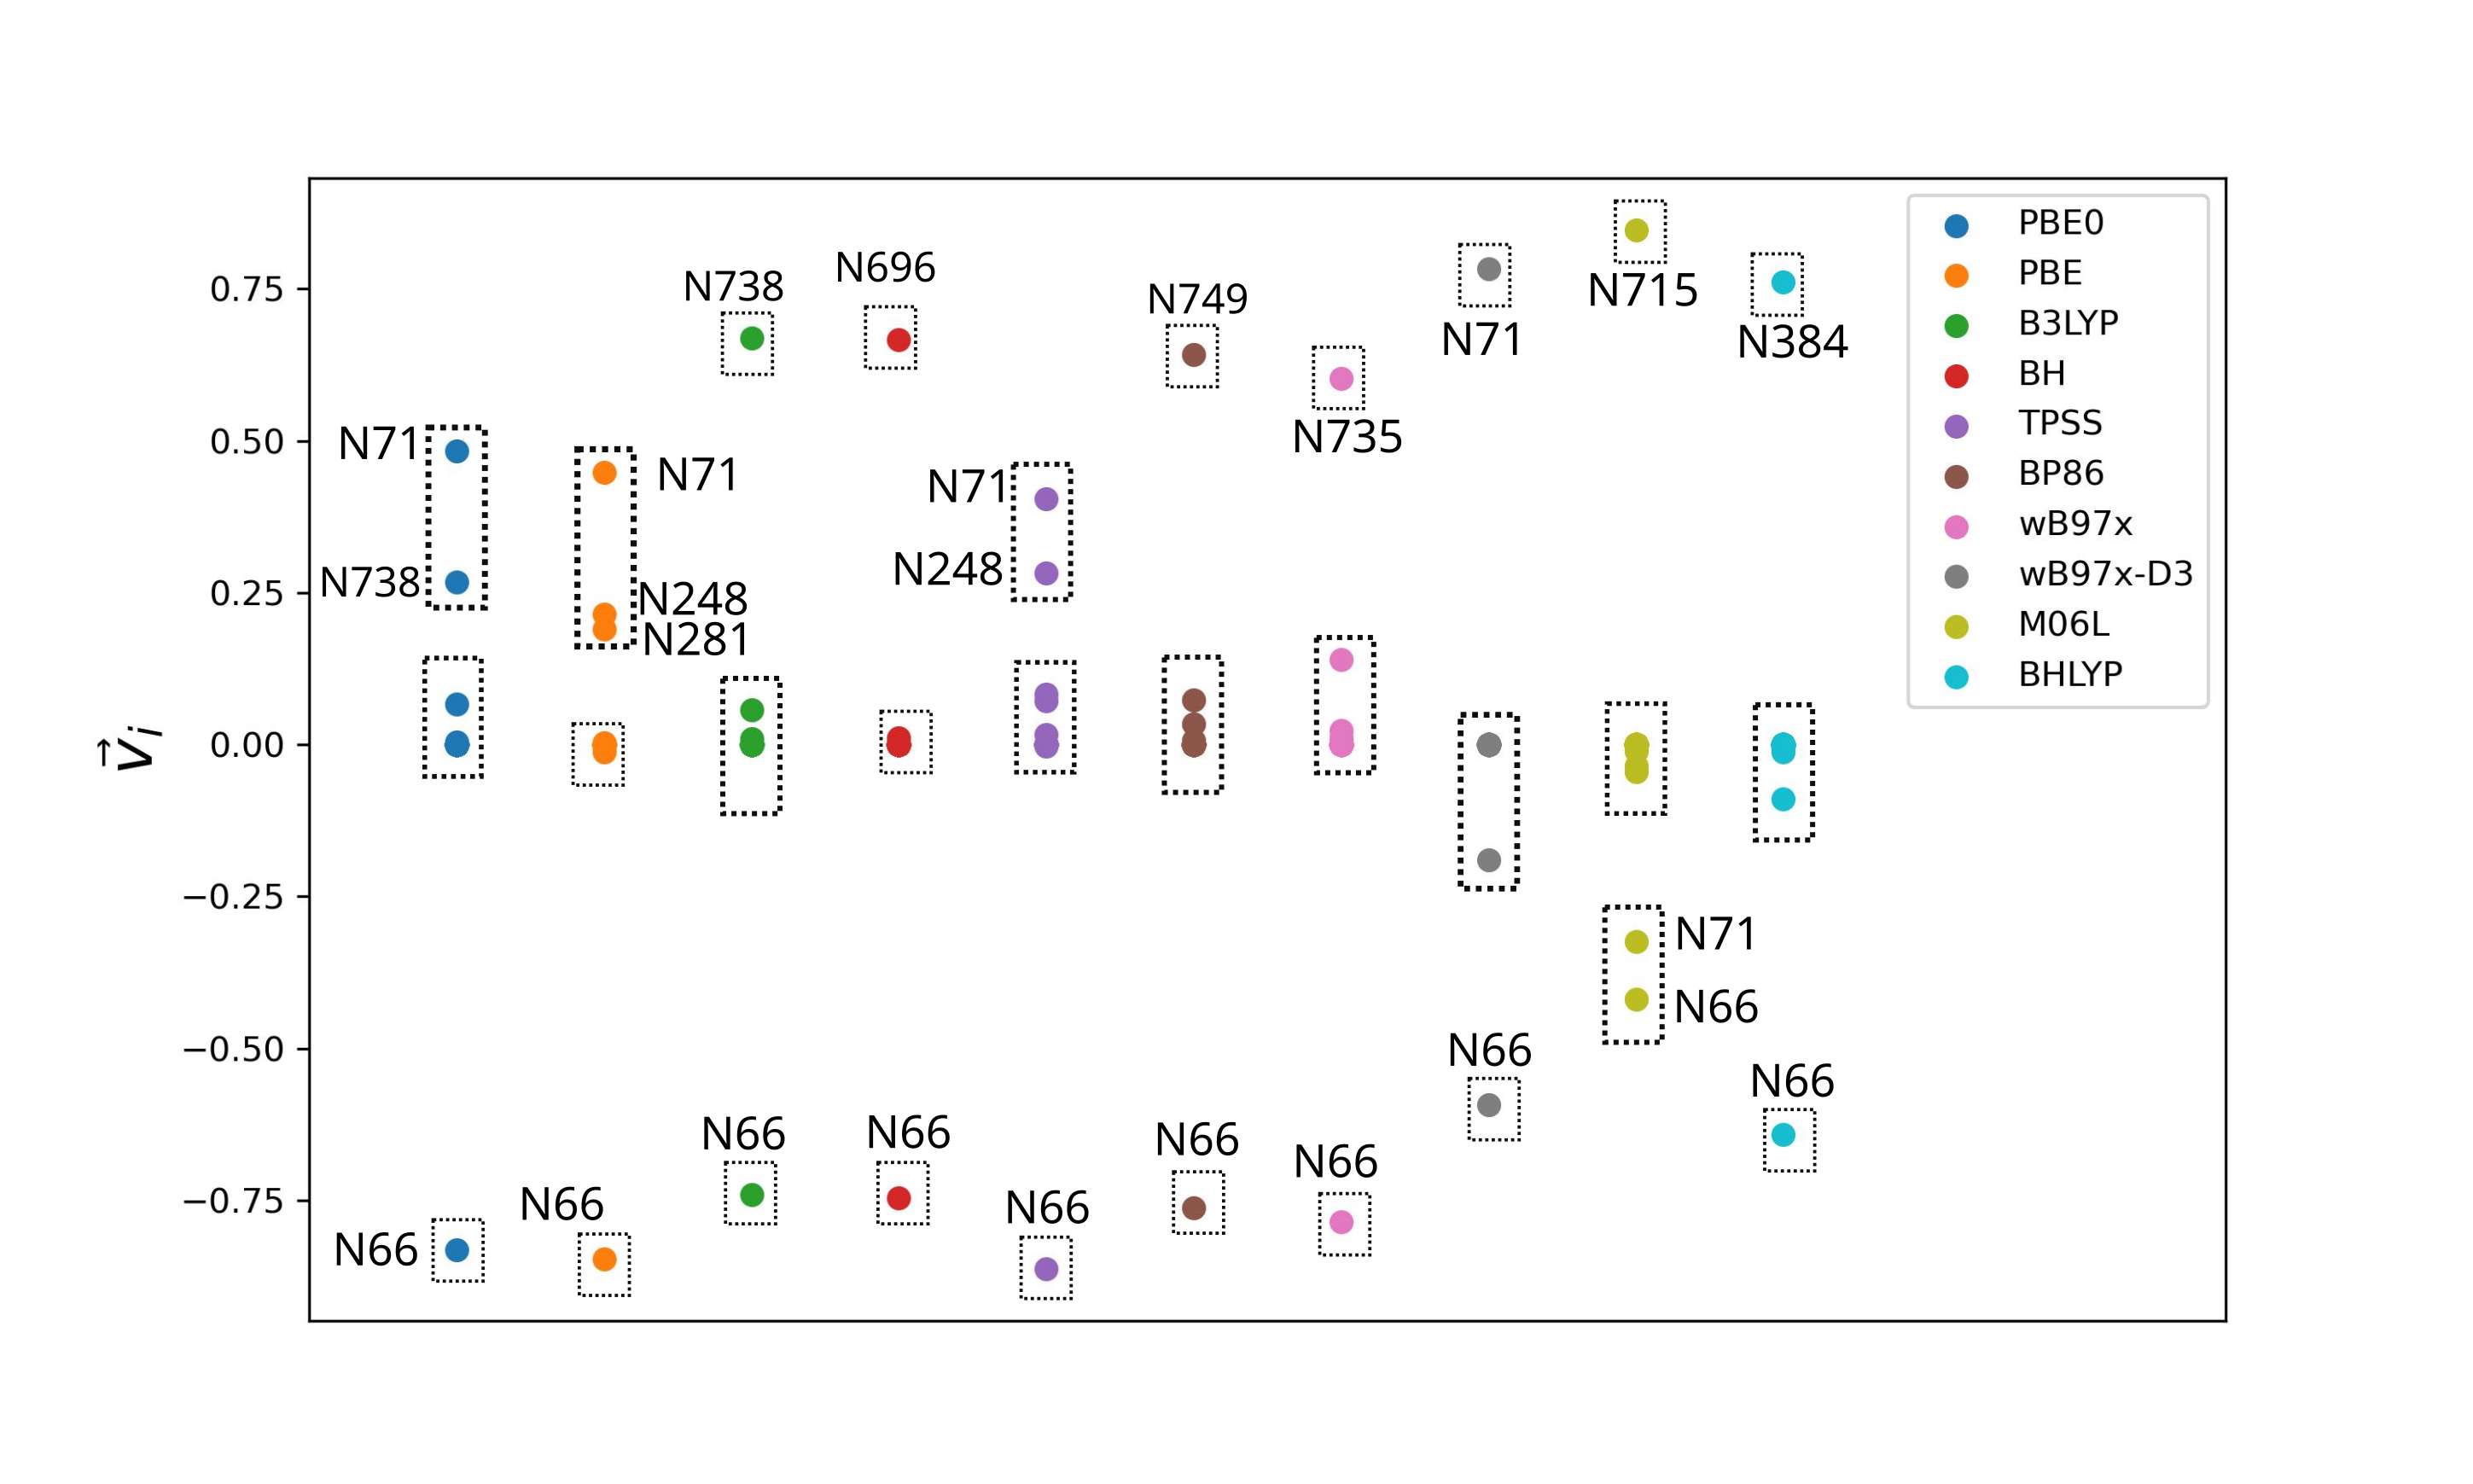
\includegraphics[width=0.8\textwidth]{figs/fig_2ndVecLw.png}
    \caption{Scatter plot of the eigen vector entries $\Vec{v}_i$ of $L_W$ for various $f$ indicated by the legend and point color. 
    The numbers are node index. The dash rectangular indicates the 3-means clusters that are detected as clusters by the Kmeans Lloyd's algorithm. }
    \label{fig:2ndVecLW}
\end{figure}

\begin{figure}
    \centering
    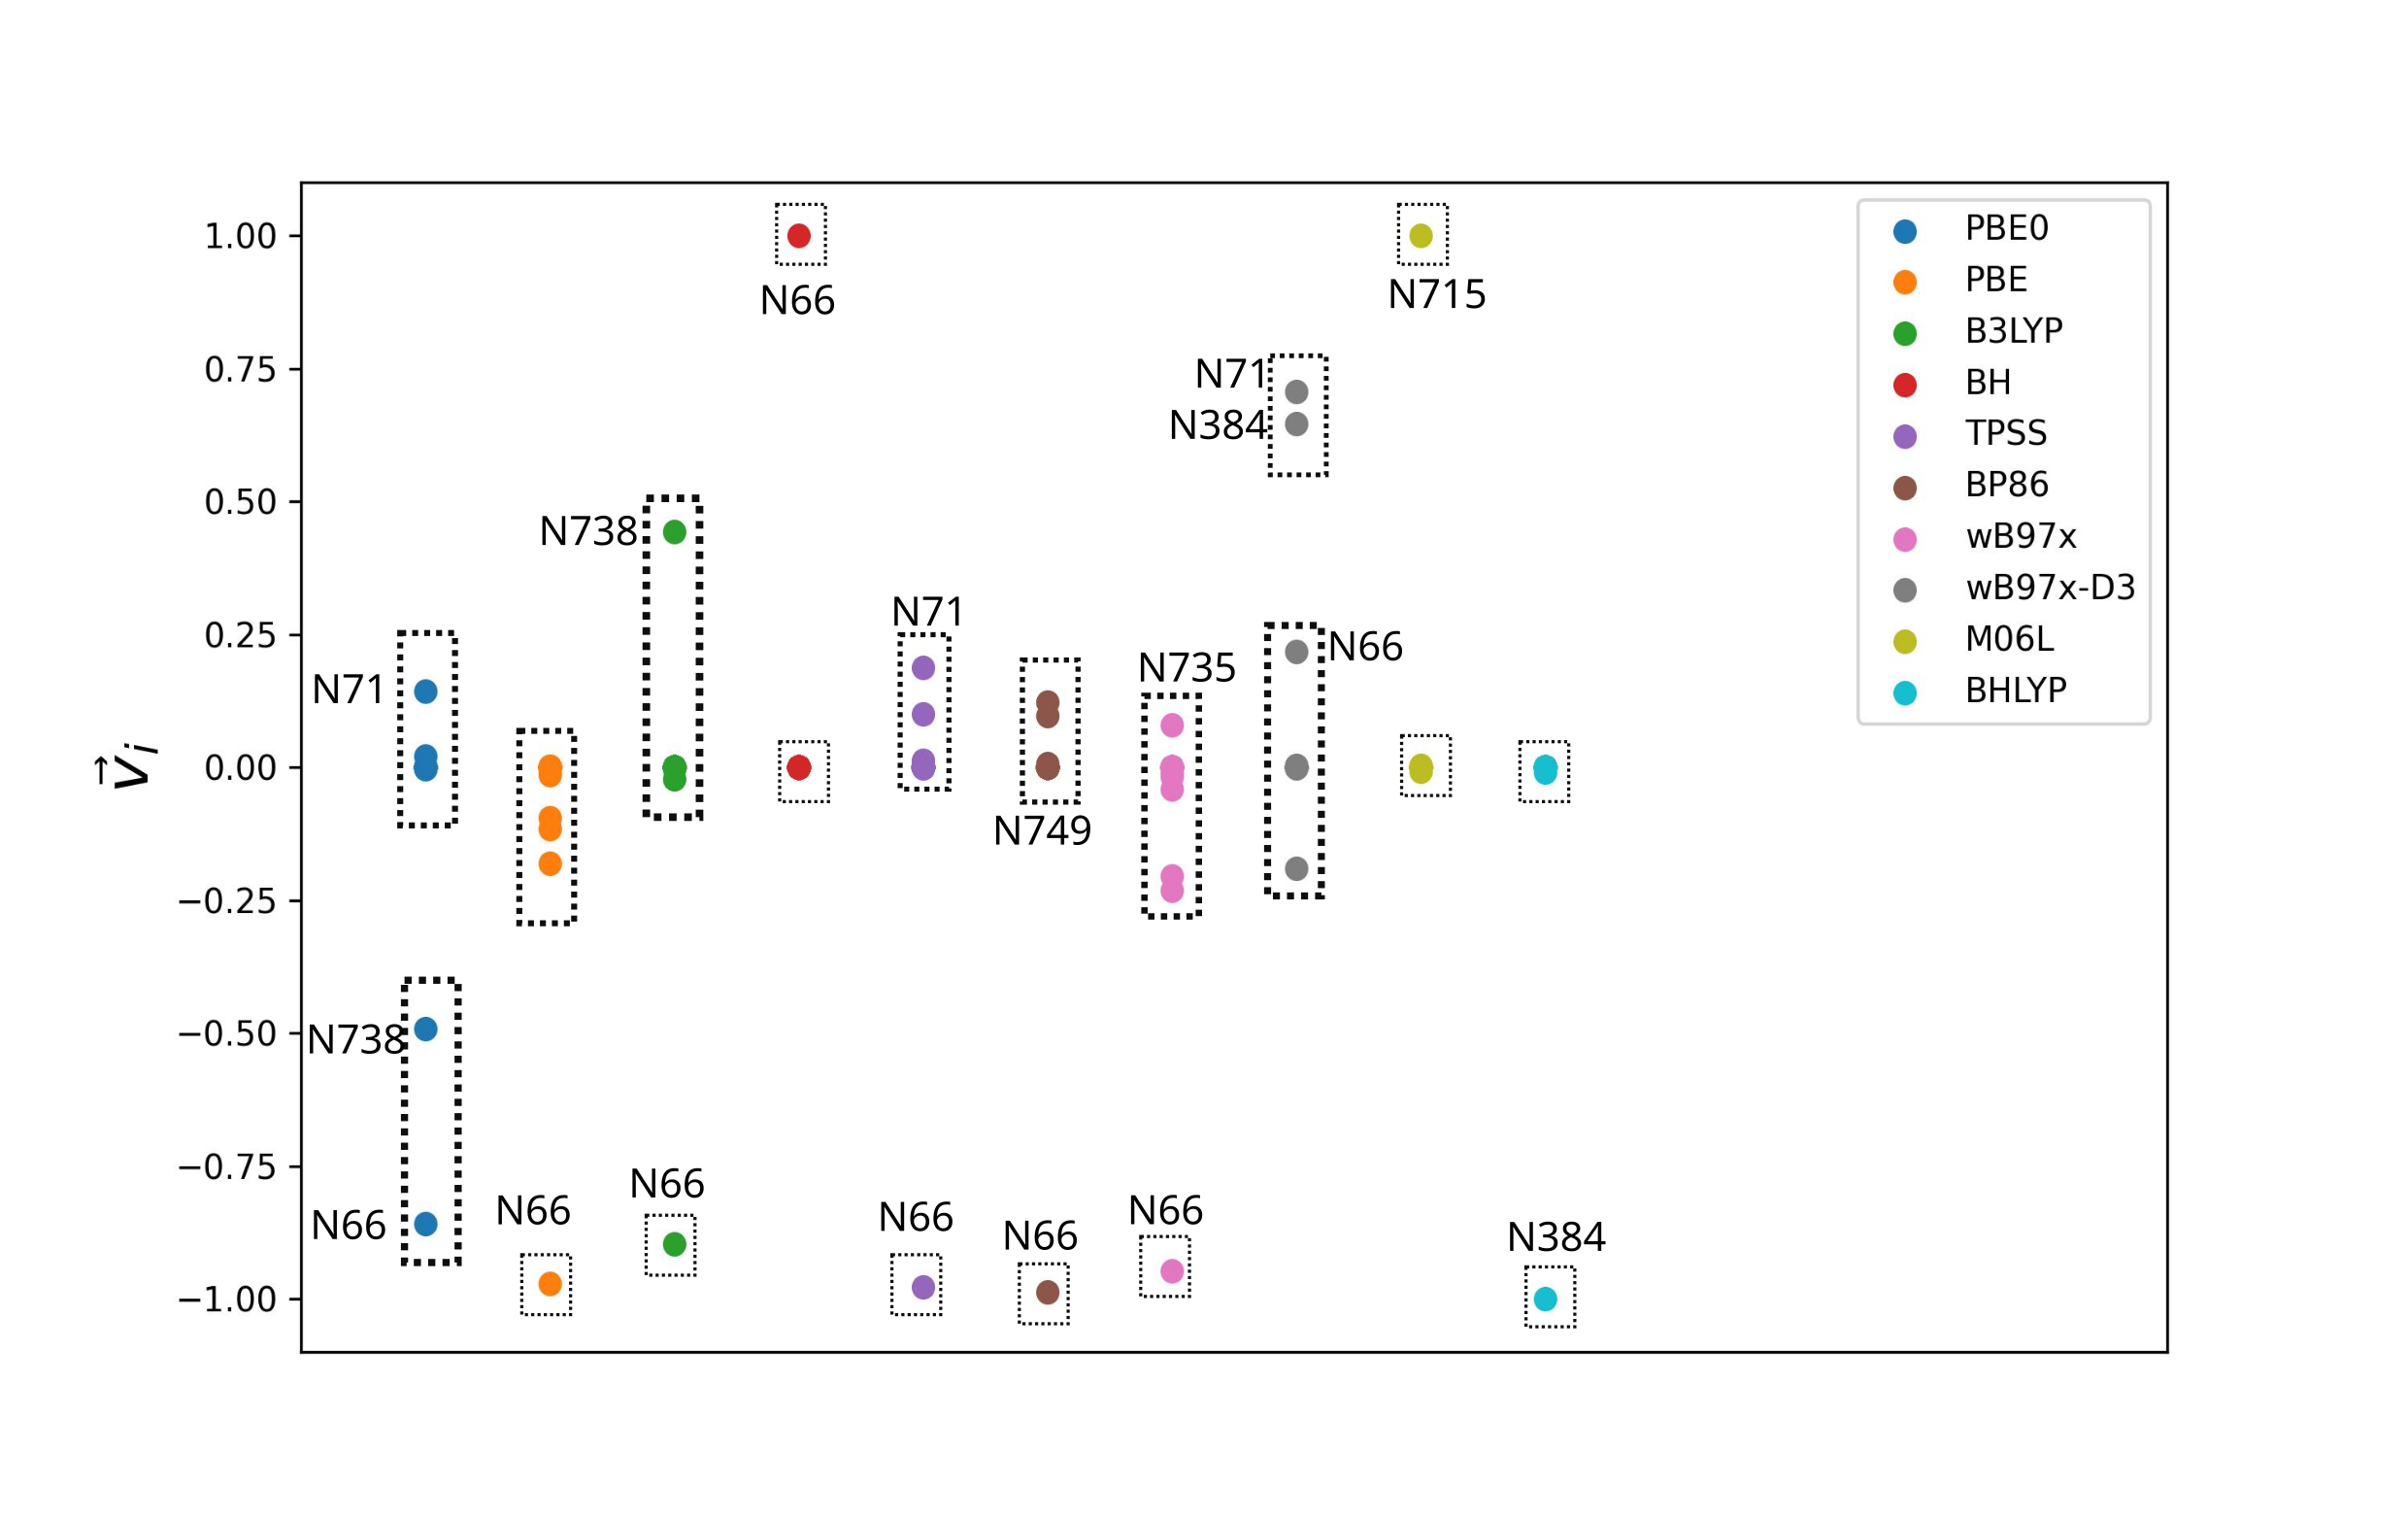
\includegraphics[width=0.8\textwidth]{figs/fig_2ndVecRW.png}
    \caption{Scatter plot of the eigen vector entries $\Vec{v}_i$ of $L_{rw}$ for various $f$ indicated by the legend and point color. 
    The numbers are node index. The dash rectangular indicates the 3-means clusters that are detected as clusters by the Kmeans Lloyd's algorithm.  }
    \label{fig:2ndVecRW}
\end{figure}


Figure \ref{fig:fig_Z_ToF} shows scatter plots of K-means clustering partition cost $Z_{2c}, Z_{3c}$ versus ToF. For the normal Laplacian $L_w$, $Z_{2c}$ is not correlated with the ToF, but $Z_{3c}$ is. For the Random-walk Laplacian, both $Z_{2c}$ and $Z_{3c}$ show a strong correlation with ToF. Thus, the clustering cost function indicates the speed of charge dynamics as measured by ToF.

\begin{figure}
    \centering
    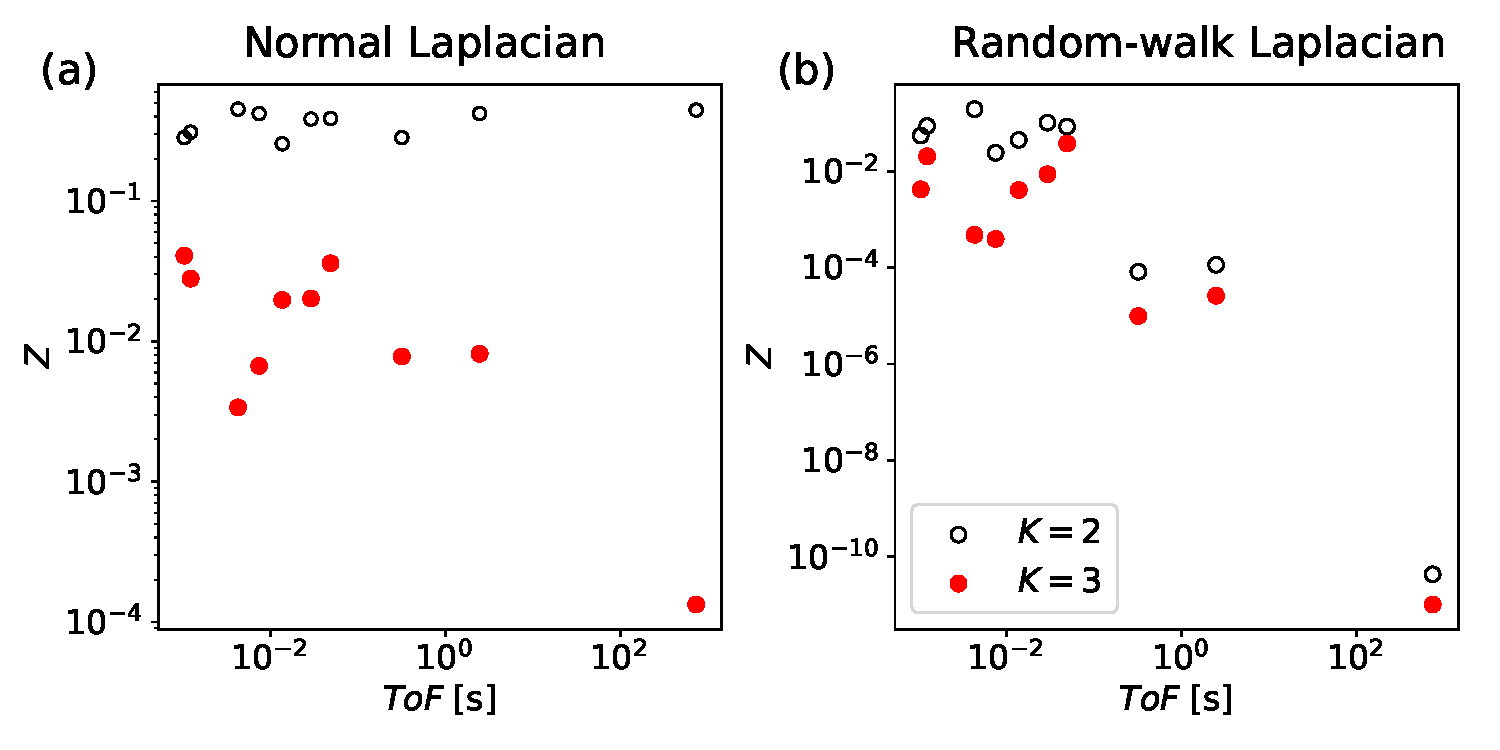
\includegraphics[width=0.9\textwidth]{figs/fig_Z_ToF.pdf}
    \caption{Scatter plot of $Z$ vs $\text{ToF}$. (a): K-means partition of the second eigenvector of $L_W$ for $K=2$ and $K=3$ (b) K-means partition of the second eigenvector of $L_{RW}$ for $K=2$ and $K=3$}
    \label{fig:fig_Z_ToF}
\end{figure} 


\textbf{Point7:} Now that the ToF has a large range, we want to know which ToF to trust.  And for application purposes, a very important message is to know what the range of ToF will give a 90\% confidence level. 

Since we do not really know the exchange-correlation potential, we assume that for each molecule, the uncertainty in its energy $E_i$ is represented by a normal distribution $E_i \in N(\bar{E_i},\sigma(E_i))$. Normal distribution is used because the normal distribution encodes the maximum amount of uncertainty over the real numbers out of all possible probability distributions with the same variance. 
So the normal distribution inserts the least amount of prior knowledge into our model. 
So we experiment: 

\textbf{Point8:} For each molecule energy $E_i$, we use maximum likelihood estimation to obtain the $N(\bar{E_i},\sigma(E_i))$. Then use sample a set of $E_i$ and calculate the ToF, with $\lambda,J_{i,j}$ fixed at the average values. 
Repeat the $E_i$ sampling and ToF calculation for 100000 times, and plot ToF distribution. This process is called the Monte Carlo sampling. 

Similarly, for $\lambda,J_{i,j}$, we perform the Monte Carlo sampling as been done for $E_i$. The resulting ToF is shown in Fig.\ref{fig:ToFs}.

\begin{figure}
    \centering
    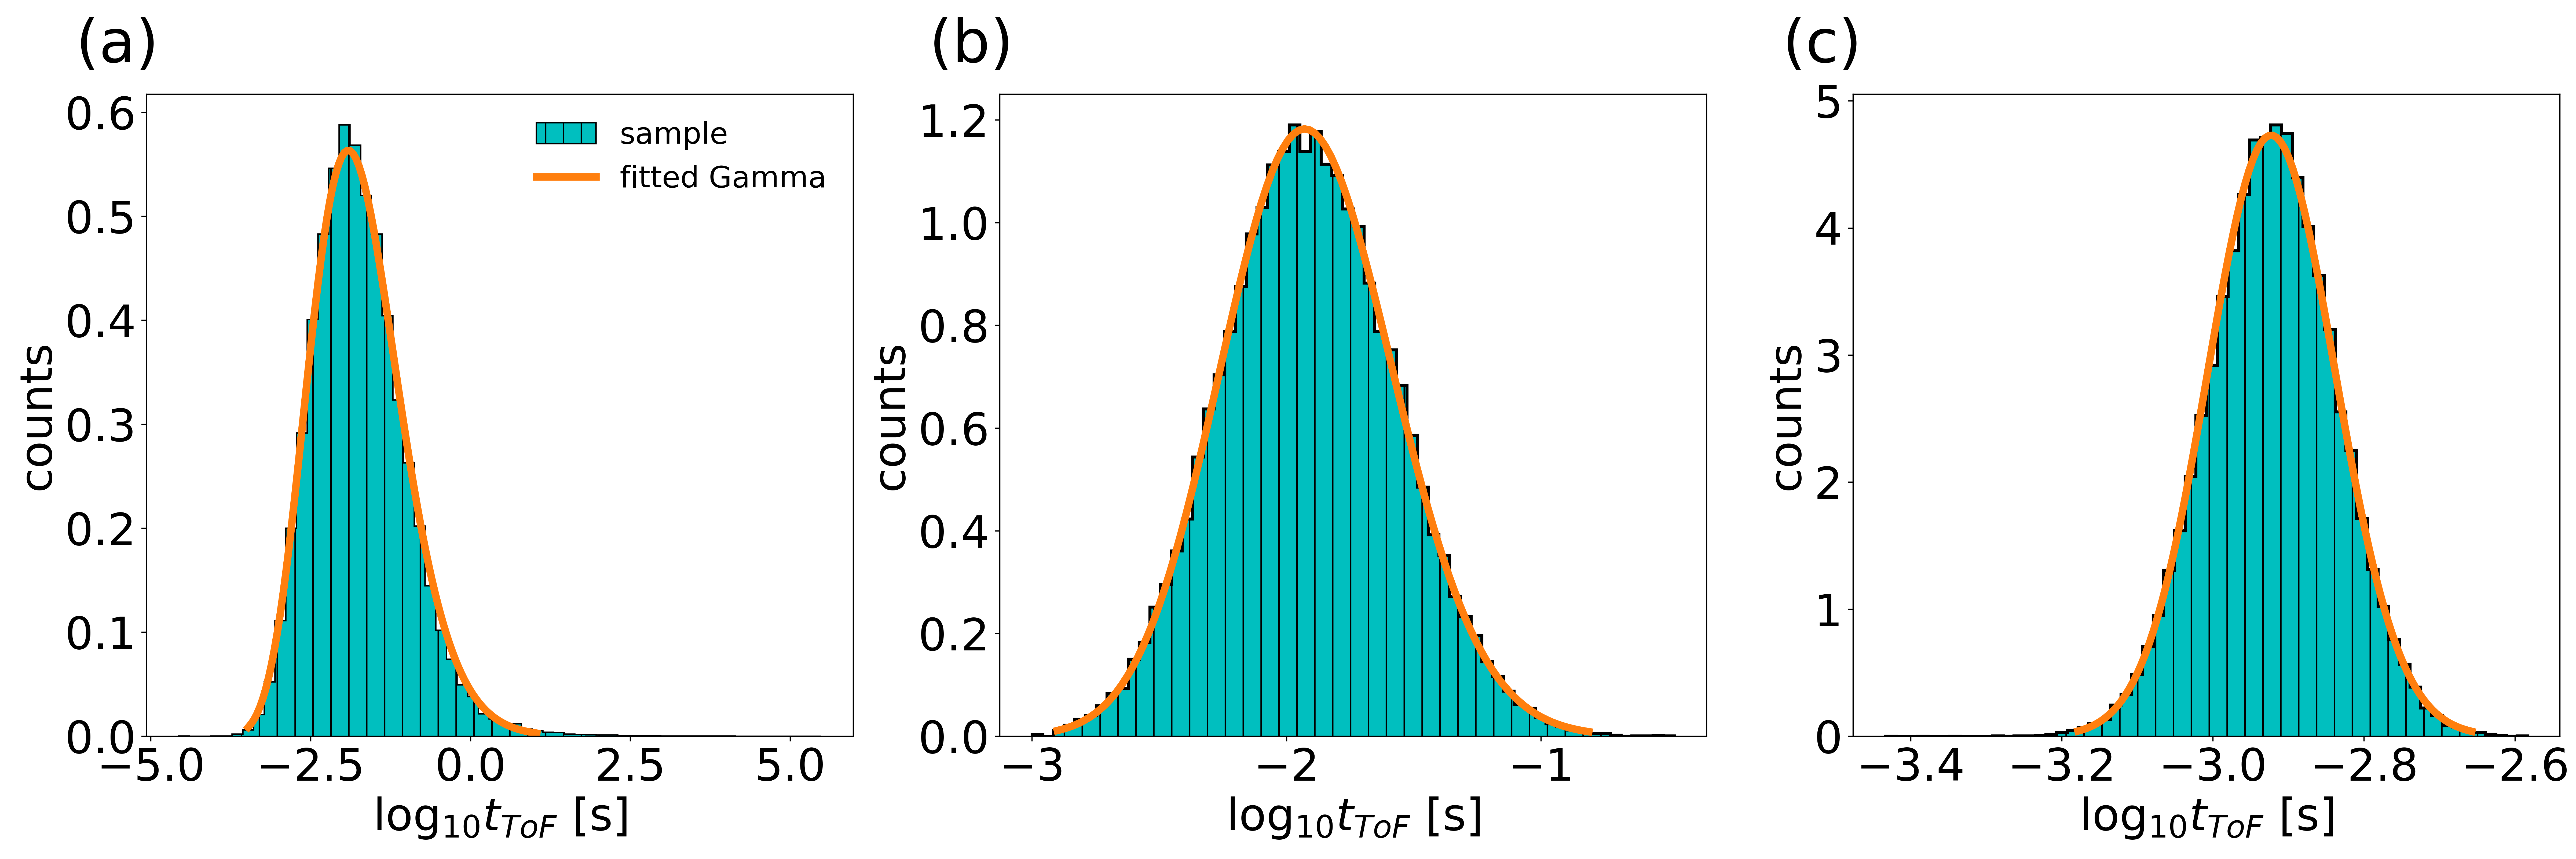
\includegraphics[width=0.9\textwidth]{figs/fig_mle.png}
    \caption{(a)The ToF distribution for 100000 samples where each $E_i$ is drawn from $N(\bar{E}_i,\sigma(E_i))$. The red curve is fitted to a gamma distribution. (b)The ToF distribution for 100000 samples where each $\lambda$ is drawn from $N(\bar{\lambda},\sigma(\lambda))$.(c)The ToF distribution for 100000 samples when each $J_{i,j}$ is drawn from $N(\bar{J_{i,j}},\sigma(J_{i,j}))$.}
    \label{fig:ToFs}
\end{figure} 

This figure shows that ToF is more sensitive to change in $E_i$ and least sensitive to $J_{i,j}$, even though from the scatter plots Fig.\ref{fig:scatterJ} the $J_{i,j}$ has a very large magnitude deviation. 

The dataset of $\log_{10}(\text{ToF})$ can be well-fitted to a Gamma distribution. 
The statistical calculation has results:
\begin{itemize}
    \item When $E_i \in N(\bar{E_i},\sigma(E_i))$, the $\log_{10}(\text{ToF})$ has mean -1.73 and a standard deviation of 0.73.
    \item When $\lambda \in N(\bar{\lambda},\sigma(\lambda))$, the $\log_{10}(\text{ToF})$ has mean -1.91 and a standard deviation of 0.34.
    \item When $J_{i,j} \in N(\bar{J_{i,j}},\sigma(J_{i,j}))$, the $\log_{10}(\text{ToF})$ has mean -2.92 and a standard deviation of 0.08.
\end{itemize}

When we use $E_i \in N(\bar{E_i},\sigma(E_i))$, $\lambda \in N(\bar{\lambda},\sigma(\lambda))$, $J_{i,j} \in N(\bar{J_{i,j}},\sigma(J_{i,j}))$ at the same to perform the Monte Carlo sampling of ToF calculation, the ToF is shown in Fig.\ref{fig:ToFs2}. the $\log_{10}(\text{ToF})$ has mean -2.72 and a standard deviation of 0.80. To obtain a 90\% confidence level, then $-3.93 < \log_{10}(\text{ToF}) < -1.30$.
\begin{figure}
    \centering
    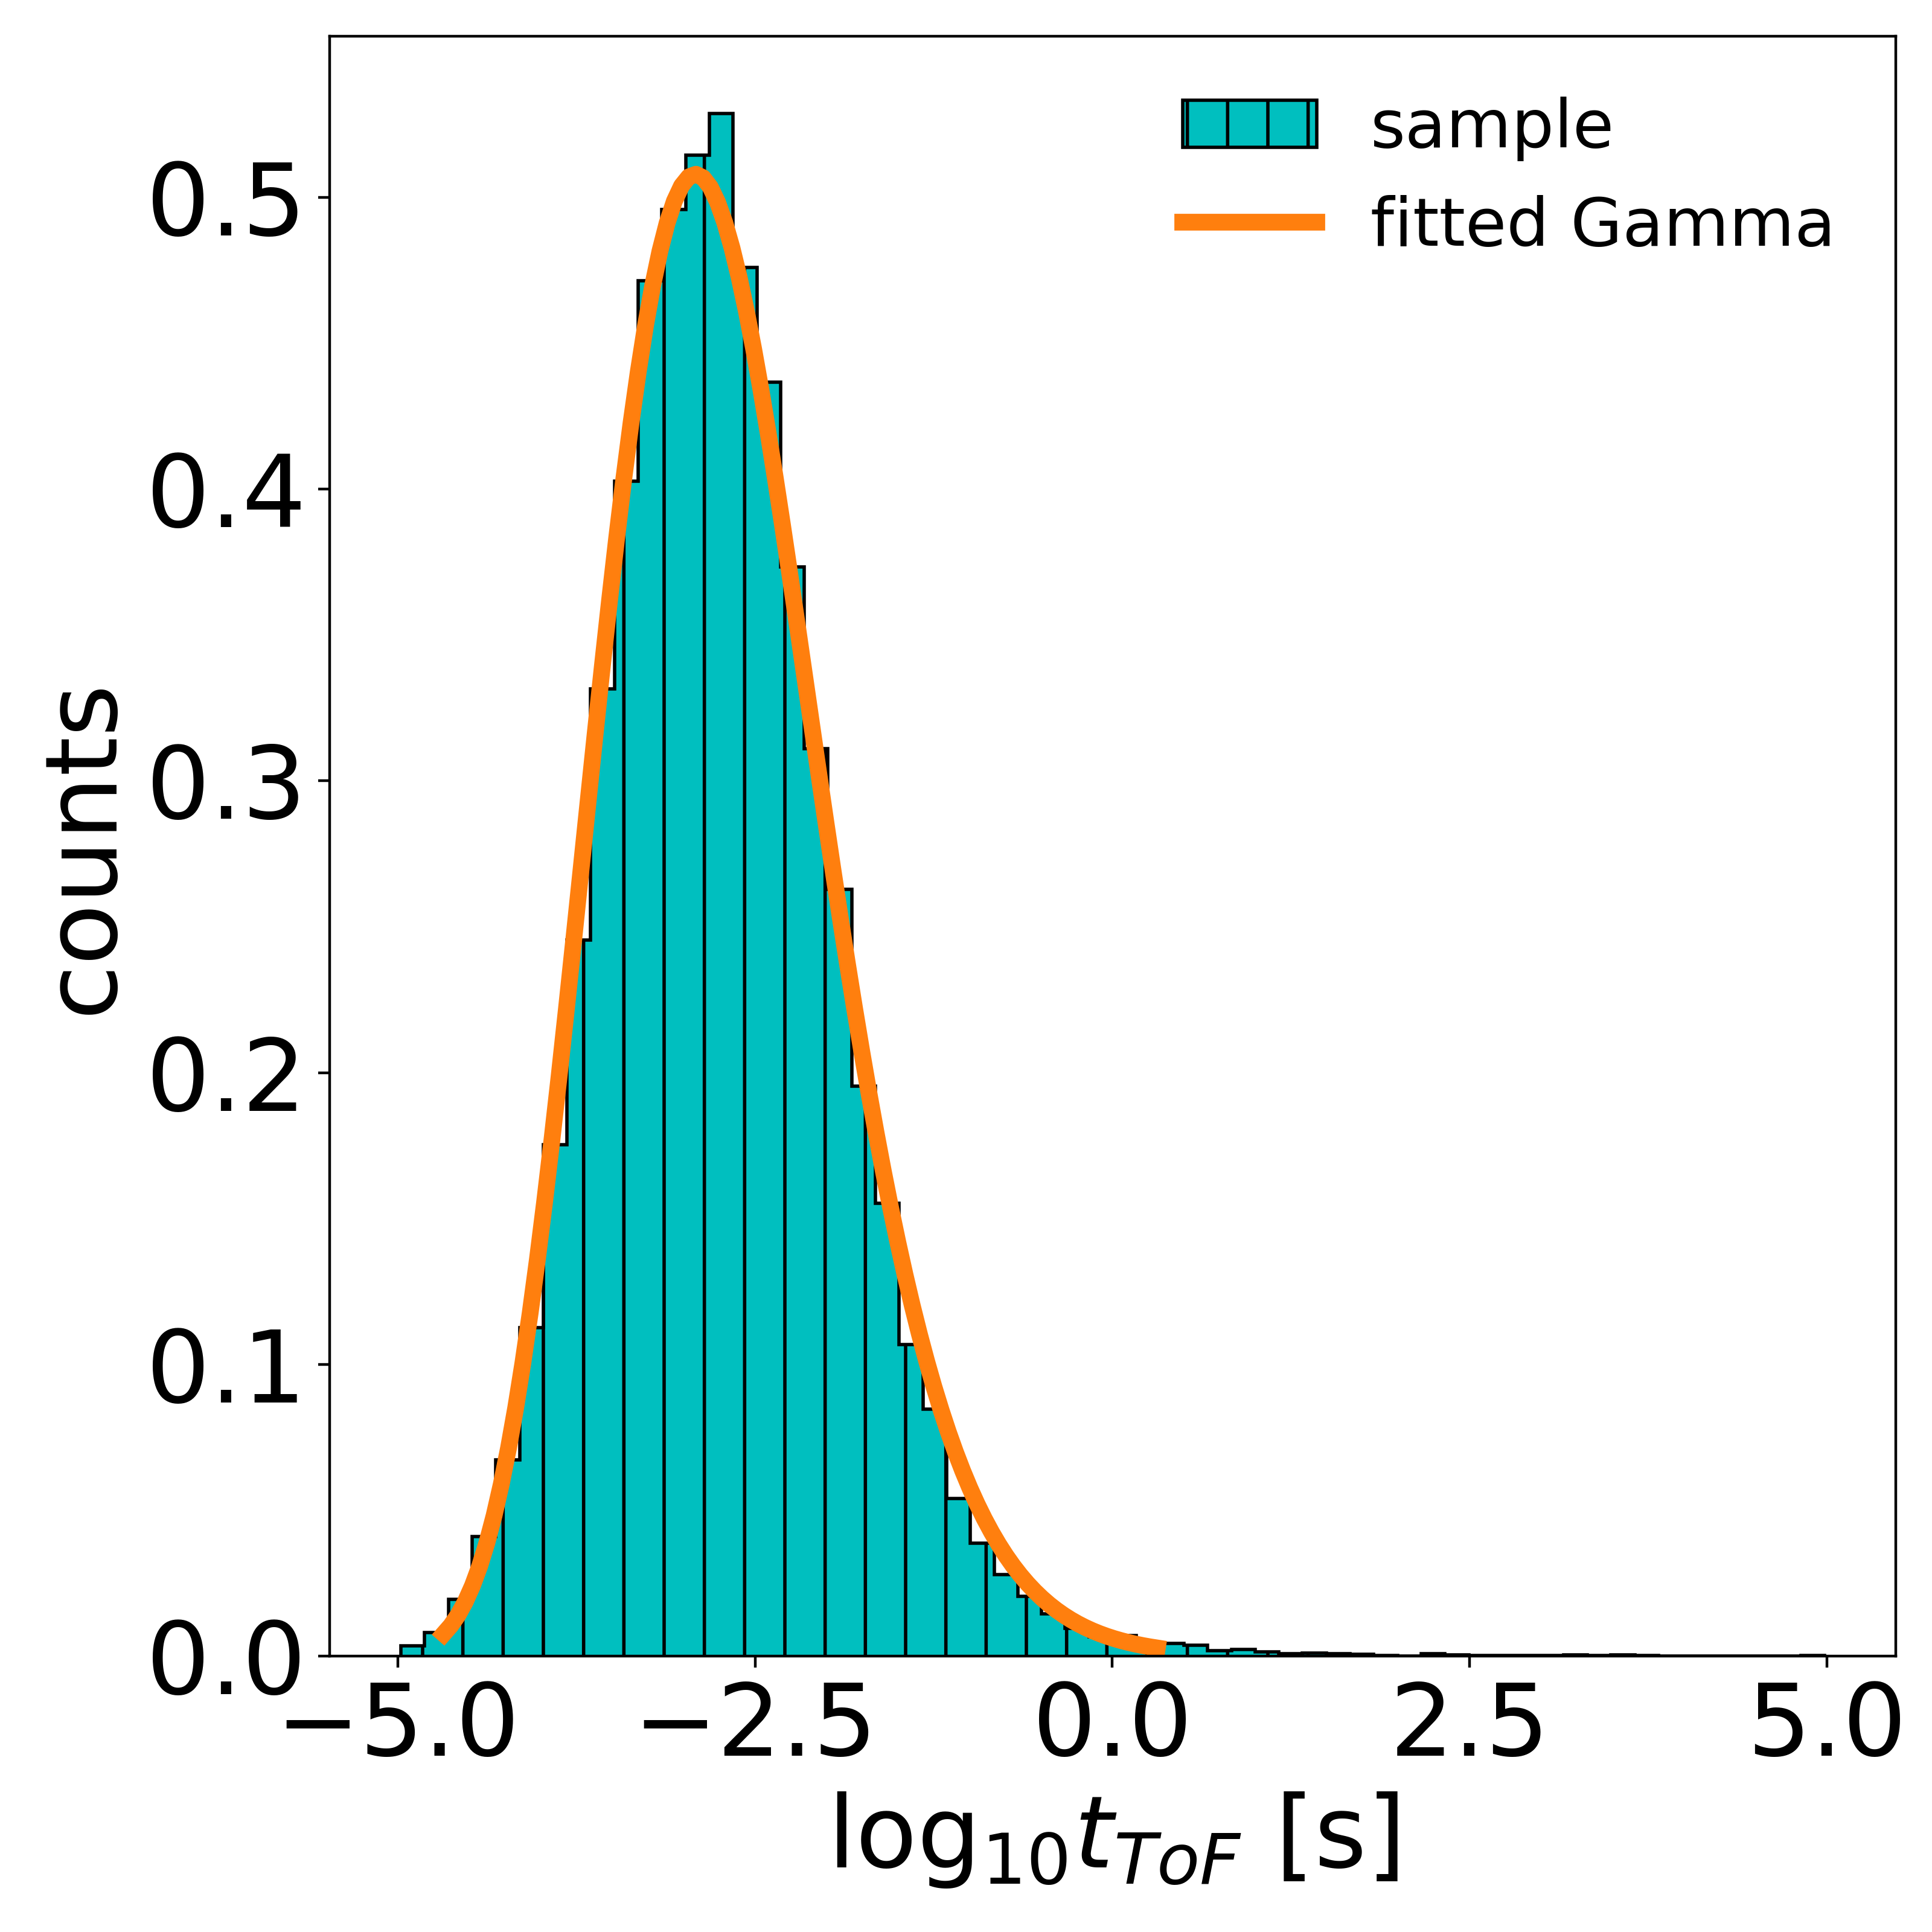
\includegraphics[width=0.6\textwidth]{figs/fig_mle2.png}
    \caption{The ToF distribution for 100000 samples where each $E_i$ is drawn from $N(\bar{E}_i,\sigma(E_i))$, $\lambda$ is drawn from $N(\bar{\lambda},\sigma(\lambda))$, and each $J_{i,j}$ is drawn from $N(\bar{J_{i,j}},\sigma(J_{i,j}))$. The red curve is fitted to a gamma distribution.}
    \label{fig:ToFs2}
\end{figure} 

%\bibliographystyle{unsrt}
%\bibliography{references}

\end{document}
